\documentclass{article}
\usepackage[utf8]{inputenc}
\usepackage[utf8, left=2.5cm, right=2.5cm, top=2.5cm, bottom=2.5cm]{geometry}
\usepackage[english]{babel}
\setlength{\parindent}{2em}
\setlength{\parskip}{1em}
\renewcommand{\baselinestretch}{1}
\usepackage{graphicx}
\usepackage{gensymb}
\usepackage{natbib}
\usepackage{amssymb}
\usepackage{xcolor}
\usepackage{wasysym}

\title{Tidal Evolution of the Earth-Moon System}
\author{Patricia Golaszewska}
\date{May $14^{th}$ 2021}
\begin{document}

\maketitle

\newpage

\begin{center}
    \section*{Introduction}
\end{center}

This project sets out to model the tidal evolution of the Earth-Moon system. The evolution of this system can be modelled using a set of ordinary differential equations:

\begin{equation}
   \frac{dL_{\oplus}}{dt} = T_{\odot}
\end{equation}

\begin{equation}
   \frac{dS_{\oplus}}{dt} = -T_{\odot} - T_{\leftmoon}
\end{equation}

\begin{equation}
   \frac{dL_{\leftmoon}}{dt} = T_{\leftmoon}
\end{equation}

The ultimate goal is to integrate these ODEs numerically using python. This allows us to model the tidal evolution of the Earth-Moon system; from initial impact to the present day. As discussed in the project outline, tidal forces have an effect on the tides. Our understanding of this phenomenon is a combination of the effects of the spin angular momentum of Earth, and the orbital angular momentum of the Sun and the moon. This then motivates the choice of the set of ODEs used in this project.


\begin{center}
    \section*{Methods}
\end{center}

We are first tasked with establishing various quantities which are used throughout the project. Due to the majority of quantities being provided in cgs units, this was the chosen unit system. Other values were converted in order to conform to this unit system.

Calculations could then be made by using the mathematical abilities of python. This allowed us to then calculate the values we'll need to feed into our integrator later on. Thus, we could calculate the numerical values of timescales associated with our three ODEs, their initial conditions, and their RHS. 

Using the scipy.integrate package and the dopri5 integrator, we could then combine our initial conditions with our ODEs following the format discussed in CTA200H lectures. Because we need to integrate into the past, a negative set of time values was chosen, ranging from the present day (0) to billions of years in the past. According to the model, the moon formed roughly 1.5 billion years ago, however, there is scientific evidence that the moon is much older than that.

Using the result of this integration, we could then analyze the evolution of the moons formation. The giant impact hypothesis is generally regarded as the leading theory in the formation of our moon. Our model allows for us to integrate into the past when the Earth and the object that would become our moon collided. At this point, their separation distance was 0 and grew over time to its present value. Thus, indexing our arrays allows us to find the time which the model predicts that the moon formed. As time moved forward, the semimajor axis expanded, and that expansion is depicted visually in Figure 1.

\begin{figure}[htp]
    \centering
    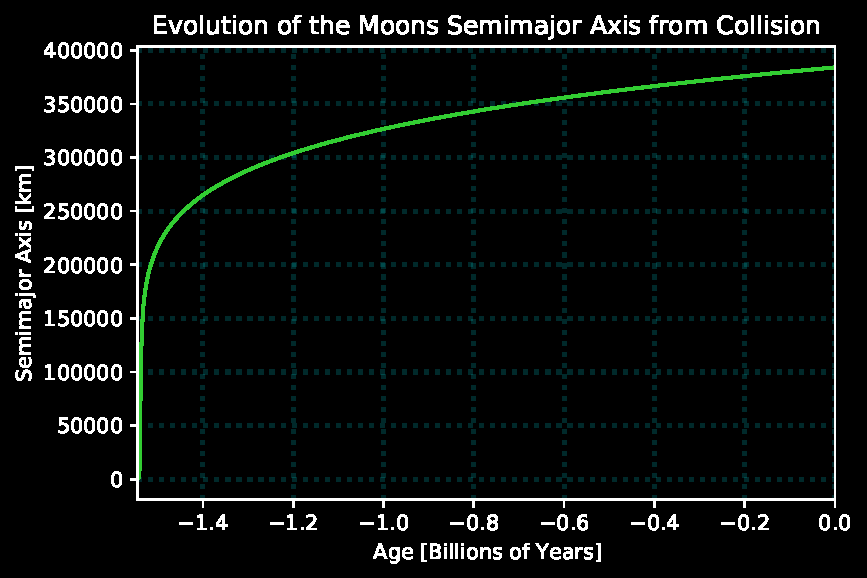
\includegraphics[width=12cm]{Q6.pdf}
    \caption{Change in the semimajor axis of the moon over time.}
    \label{fig:Q6}
\end{figure}

If the moon formed at the Roche radius (at approximatley 9496 km), then the length of day would be approximately 4 hours long. As the system stabilized over time, the length of day became longer. This is depicted visually in Figure 2. 

\begin{figure}[htp]
    \centering
    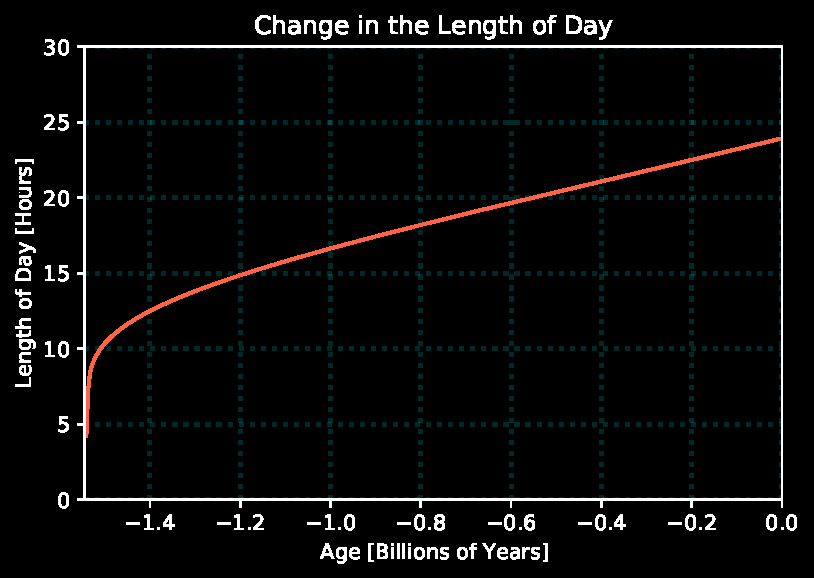
\includegraphics[width=12cm]{Q7.pdf}
    \caption{Change in the length of day on Earth over time.}
    \label{fig:Q7}
\end{figure}

Issues surrounding this model arise from the incorrect age we get for our system. I suspect that there may be issues with how our model predicts the evolution of this system, and possibly doesn't account for the conditions at impact.

Firstly, I do not believe that this model allows for the moon to go through the process of mass accretion. This process would change the dynamics of the system over time as the gravitational effects change.

Second, I believe that this model assumes that the Earth-Moon system has been tidally locked from impact. This is an extension of the point made above; the dynamics of this system age the Earth-Moon system based on the tidal evolution. However, if the moon spent a period of time in asynchronous rotation, this model doesn't capture this.

I believe that this model interprets the collision as formation, which isn't necessarily true. The moon would have began it's formation at some distance away (i.e possibly the Roche radius) versus at impact.

Additional inconsistencies may be caused by changes in the eccentricity and alignment of the moons orbit, as well as external gravitational influences. Stabilization and tidal-locking may also result in changes in the energy in this system, which could have influenced the evolution of our system. 

These reasons are listed in the order of what I assume to be the most reasonable assumption. My primary concern is that the initial dynamics of the system differ than those observed today, and they are not accounted for in the scope of this project.

\end{document}
